\documentclass[a4paper,
               %boxit,
               %titlepage,   % separate title page
               %refpage      % separate references
              ]{jacow}

\ifboolexpr{bool{xetex} or bool{luatex}} % test for XeTeX/LuaTeX
 {}                                      % input encoding is utf8 by default
 {\usepackage[utf8]{inputenc}}           % switch to utf8

\usepackage{graphicx, subfigure}
\usepackage{booktabs}


\begin{document}
\title{BEAM COUPLING IMPEDANCE OF THE NEW BEAM SCREEN OF THE LHC INJECTION KICKER MAGNETS}
\author{H. Day\thanks{hugo.day@hep.manchester.ac.uk}$^{\dagger}$, M.J. Barnes$^{\dagger}$, F. Caspers$^{\dagger}$, E. Métral$^{\dagger}$, B. Salvant$^{\dagger}$, J. Uythoven$^{\dagger}$ \\
$\dagger$ CERN, Switzerland
}

\maketitle 


\begin{abstract}
The LHC injection kicker magnets experienced significant beam induced heating of the ferrite yoke, with high intensity beam circulating for many hours, during operation of the LHC in 2011 and 2012. The causes of this beam coupling impedance were studied in depth and an improved beam screen implemented to reduce the impedance. Results of measurements and simulations of the new beam screen design are presented in this paper: these are used to predict power loss and temperature of the ferrite yoke for operation after long shutdown 1 and for proposed HL-LHC operational parameters.
\end{abstract}

\section{Introduction}

During the 2011 and 2012 runs of the LHC, high temperatures were observed in several devices in the LHC  \cite{metral_cham2012}, a critical piece being the LHC injection kicker magnets (MKIs) Fig.~\ref{fig:mkiStruct}, which were attributed to beam-induced heating due to high power loss from the interaction of the circulating beam with the longitudinal beam coupling impedance. This heating was observed to raise the temperature of the ferrite yoke of one of the MKIs above its Curie point during fills, thereby necessitating waiting times of several hours for the ferrite to cool before safe injection could be carried out \cite{mki-heating}. A magnet with an improved beam screen was inserted during technical stop 3 (TS3) (23/09/12-27/09/12), replacing the MKI8D which was measured to have the highest temperature \cite{mki-heatingTemp}; the replacement magnet was subsequently measured to have the lowest temperature of all magnets.

Building on this success a new design has been proposed to satisfy competing needs of low rates of electrical breakdown during magnet pulsing and a low beam coupling impedance to reduce the power lost into the structure by wakefields; in addition to meeting strict requirements for magnet operation for field rise time and flat top stability \cite{mkiUpgrade}. 

\begin{figure}
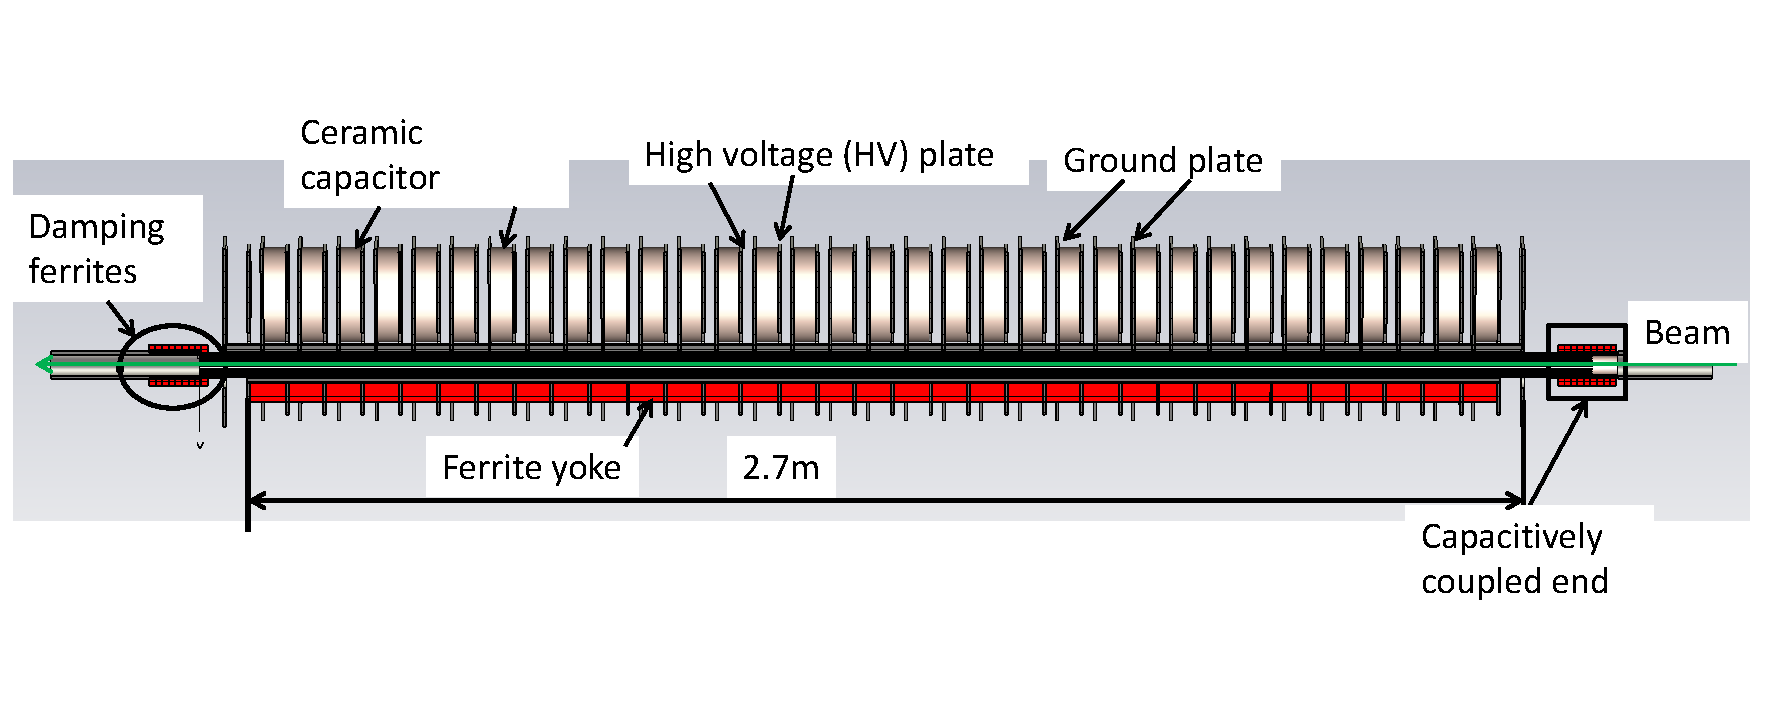
\includegraphics[width=0.5\textwidth]{MKICrossSectionYZ.pdf}
\caption{Structure of the injection kicker magnets.}
\label{fig:mkiStruct}
\end{figure}

\section{New Beam Screen Design}

The new design involves a redesign of the capacitively coupled end of the beam screen, intended to reduce the electrical field due to the induced potentials on the screen conductors during magnet pulsing. This reduced electric field reduces the possibility of surface breakdown on the internal face of the beam screen allowing additional beam screens to be inserted where previously they had been removed due to being located in regions of high electric field Fig.~\ref{fig:beamScreenCross} providing complete screening of the ferrite yoke of the magnet. See \cite{mki-ElecBreakdown} for more information on behaviour relating to surface flashover. 

\begin{figure}
\begin{center}
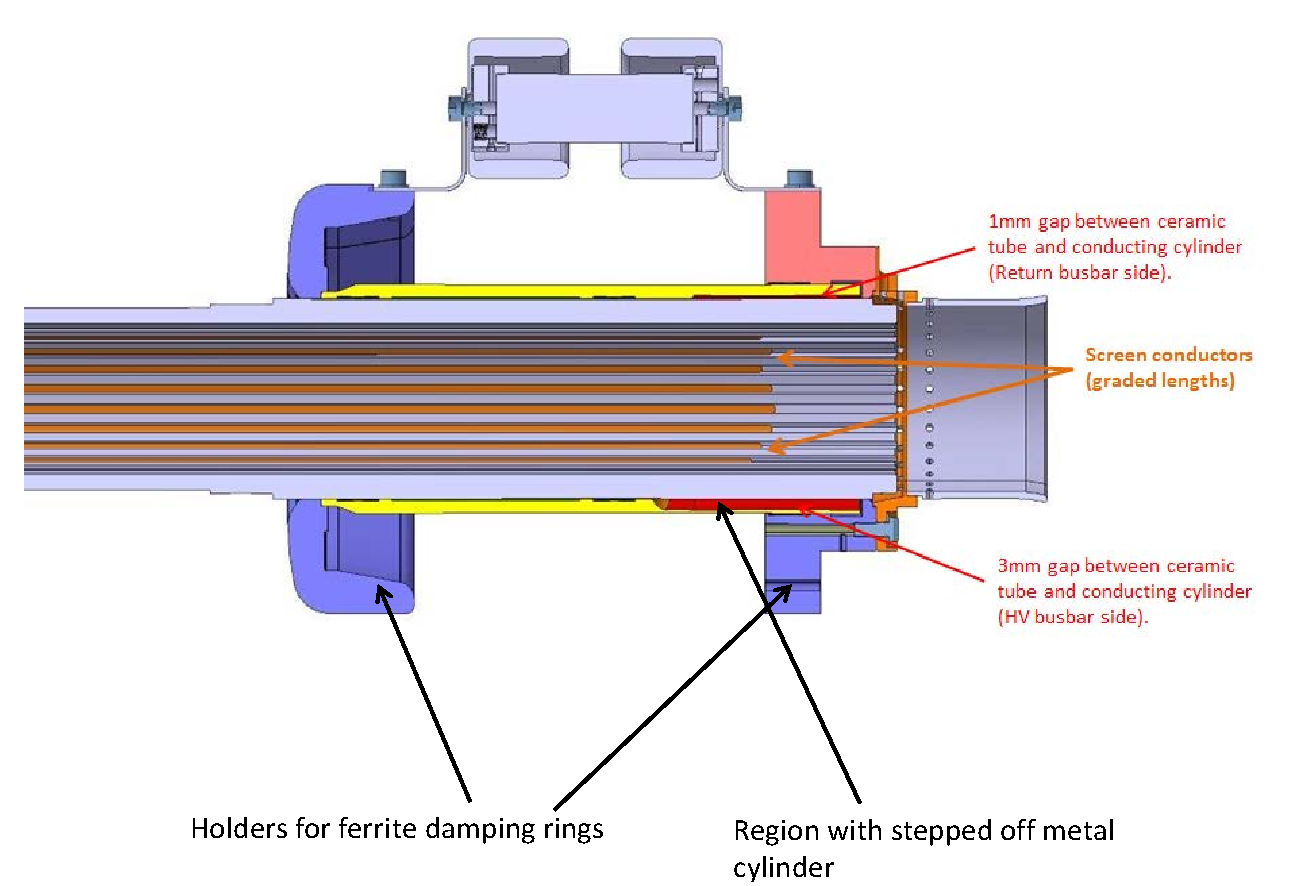
\includegraphics[width=0.45\textwidth]{beamScreenCrossSectionLabelled.pdf}
\caption{Cross section of the new beam screen design}
\label{fig:beamScreenCross}
\end{center}
\end{figure}



\section{Impedance Measurements}

In order to observe the effect of manufacutring tolerences between magnets and as part of the campaign to characterise the impedance of all devices placed into the LHC each of the MKIs with the new beam screen has it's longitudinal beam coupling impedance measured during assembly. These measurements are carried out using the resonant coaxial wire method [cite], a measurement technique that turns the device under test (DUT) into a coaxial resonator with a weak external coupling. This allows very sensitive measurements of the impedance of the DUT to be made, at the cost of a relatively poor frequency resolution as the measurement is of the Q-factor at the resonant frequencies of the coaxial device.

The real component of the longitudinal beam coupling impedance of an example of the new design as well as for an MKI before LS1 (with 15 screen conductors) and the MKI8D that was replaced in TS3 (with 19 screen conductors) are shown in Fig.~\ref{fig:Imp241915}. It can be seen that the new design has a substantially lower beam coupling impedance over the majority of the frequency range, with the broadband impedance seen in the case of 15 screen conductors becoming resonant in nature with 24 conductors. This is due to the improved screening of the ferrite yoke by having 24 screen conductors equally distributed around the beam screen as opposed to an arc of some 135$^{\circ}$ left unscreened when only 15 screen conductors are in place.

\begin{figure}
\caption{Real component of the longituidinal beam coupling impedance measured using the resonant coaxial wire method for the new beam screen design, the design with 15 screen conductors as was the case for most magnets prior to LS1 and the upgraded MKI8D, inserted in TS3.}
\label{fig:Imp241915}
\end{figure}

The real component of the longitudinal beam coupling impedance of the 9 MKIs upgraded with the new beam screen design to date (June 2014), measured using the resonant coaxial wire technique. It can be seen that the consistency between the magnets is very good - resonant frequencies are *Res freq +/- error*, with peak impedances of *peak +/- error* for the first measured resonance at 890MHz. This indicates that with the rigorous assembly procedure has eliminated some of the variation in the beam impedance of the MKIs prior to LS1.

\begin{figure}
\caption{Real component of the longitudinal beam coupling impedance measured using the resonant coaxial wire method for the first 9 magnets fitted with the new beam screen design. 8 are to be installed for use after LS1, with an additional 4 as spares.}
\label{fig:allNewMKIImp}
\end{figure}

To verify the simulations carried out in the design phase of the new design we compare a number of measurement methods. The resonant coaxial wire method provides very good accuracy for the measurements but relatively poor frequency resolution if only the DUT is used in the coaxial resonator; frequency data points are spaced such that $\Delta f \approx \frac{nc}{2L_{DUT}}$, where $n$ is an integer. $c$ the speed of light, $L_{DUT}$ the length of the device measured. The classical coaxial wire technique gives a frequency range determined only by the frequency points on the network analyser, however any residual mismatch in the characteristic impedance between the measurement network and the DUT will result in reflections in the system which limits the achieveable accuracy. Alternatively it's possible to use time domain gating to gate out reflected signals, however due to the varying characteristic impedance along the length of the DUT it's difficult to gate all reflections without losing sensitivity in the measurements.

\section{Power Loss}




\section{Future Plans}
%Title format - Title; Authors; Affiliation; conference
%Abstract - Copied from submitted abstract (maybe changed to represent changes in presented paper)
%Introduction
%Body of data
%Conclusion
%Acknowledgements
%References

% Aim of paper - To present the causes of the beam coupling impedance in the beam screen - length of overlap, thickness, screening by conductors. Expected power loss for the new screen design with present and HL-LHC parameters
% Sections:
% Introduction - Brief history of the MKI heating - reference to Mike's paper last year and this year
% Reasons for the impedance - Distinction between well screened and not well screened
% - Increasing number of screen conductors reduces effect of the ferrite
% - Dimensions of the capacitive end changing impedance profile
% - Effect of different ferrites on the 30-40MHz peak if time
% Power loss expectactions for HL-LHC, post LS1 between 15, 19 and New design
%
%
%

% Images to include
% New screen design cross section
% New screen design impedance
% Various lengths of overlap impedance and predicted resonant frequency
% 

\section{INTRODUCTION}


\begin{thebibliography}{9}

\bibitem{mkiUpgrade}
M.J. Barnes \emph{et al}., \emph{Upgrade of the LHC Injection Kicker Magnets}, IPAC'13, Shanghai, China, MOPWA030

\bibitem{metral_cham2012}
E. Métral \emph{et al}., \emph{Beam-Induced Heating/Bunch Length/RF and Lessons for 2012}, LHC Performance Workshop, Chamonix 2012, CERN-ATS-2012-069. 

\bibitem{mki-heating}
M.J. Barnes \emph{et al}., \emph{"Analysis of Measured Ferrite Heating of the LHC Injection Kickers and Proposals for Future Reduction of Temperature"}, IPAC'12, New Orleans, USA, 2012, TUPPR090.

\bibitem{mki-heatingTemp}
M.J. Barnes \emph{et al}., \emph{"Beam Induced Ferrite Heating of the LHC Injection Kickers and Proposals for Improved Cooling"}, IPAC'13, Shanghai, China, MOPWA031.

\bibitem{kicker_meas}
H. Day \emph{et al}., \emph{"Evaluation of the Beam Coupling Impedance of new Beam Screen Designs for the LHC Injection Kicker Magnets"}, IPAC'12, New Orleans, USA, 2012, WEPPR071.

\bibitem{mki-ElecBreakdown}
M.J. Barnes \emph{et al}., \emph{"Reduction of Surface Flashover of the Beam Screen of the LHC Injection Kickers"}, IPAC'13, Shanghai, China, MOPWA031.

\bibitem{cst-cite}
\texttt{http://www.cst.com}.

\bibitem{DayThesis}
PhD Thesis, H. Day, 2013.

\bibitem{LHCRF}
P. Baudrenghien \emph{et al}., \emph{"The LHC RF System - Experience with Beam Operation"}, IPAC'11, San Sebastian, 2011, MOPC054.


\end{thebibliography}
\end{document}

